\section{迭代磁共振成像重建}
在本章中,我们从一个相对简单的应用程序的背景和问题阐述开始,该应用程序传统上受到主流计算系统有限功能的限制。 
我们表明,并行执行不仅可以加快现有方法的速度,
而且还允许应用程序专家追求一种已知可以带来好处但之前由于计算要求过高而被忽视的方法。 
这种方法代表了一类日益重要的计算方法,这些方法从大量观测数据中得出未知值的统计最佳估计。 
我们使用这种方法中的示例算法及其实现源代码来说明开发人员如何系统地确定内核并行结构、
将变量分配到不同类型的存储器、绕过硬件的限制、验证结果并评估 性能改进。

\subsection{背景}
磁共振成像 (MRI) 通常用作一种医疗程序,可安全、无创地探测身体所有区域的生物组织的结构和功能。 
使用 MRI 生成的图像对临床和研究环境产生了深远的影响。 MRI 包括两个阶段:采集(扫描)和重建。 
在采集阶段,扫描仪沿着预定义的轨迹对 k 空间域(即空间频域或傅立叶变换域)中的数据进行采样。 
然后在重建阶段将这些样本转换为所需的图像。 直观地说,重建阶段根据从扫描仪收集的观察 k 空间数据来估计组织的形状和纹理。

MRI 的应用通常受到高噪声水平、显着的成像伪影和/或长数据采集时间的限制。 
在临床环境中,短扫描时间不仅可以提高扫描仪的吞吐量,还可以减少患者的不适,这往往会减轻与运动相关的伪影。 
高图像分辨率和保真度非常重要,因为它们可以实现病理的早期检测,从而改善患者的预后。 
然而,短扫描时间、高分辨率和高信噪比 (SNR) 的目标经常发生冲突; 一项指标的改进往往会以牺牲其他一项或两项指标为代价。 
需要新的技术突破来实现所有三个维度的同步改进。 这项研究提出了大规模并行计算提供此类突破的案例。

读者可以参考Liang 和Lauterbur (1999) 等MRI 教科书来了解MRI 背后的物理原理。 
对于本案例研究,我们将重点关注重建阶段的计算复杂性以及复杂性如何受到 k 空间采样轨迹的影响。 
MRI扫描仪使用的k空间采样轨迹可以显着影响重建图像的质量、重建算法的时间复杂度以及扫描仪获取样本所需的时间。 
等式 (17.1) 显示了将 k 空间样本与一类重建方法的重建图像相关联的公式:
$$
\widehat{m}(\mathrm{r})=\sum_{j} W\left(\mathrm{k}_{\mathrm{j}}\right) s\left(\mathrm{k}_{j }\right) e i 2 \pi \mathrm{k}_{\mathrm{j}} \mathrm{r}
$$

在等式(17.1)中,$m(\mathbf{r})$是重建图像,$s(\mathbf{k})$是测量的k空间数据,
$W(\mathbf{k})$是 考虑非均匀采样的加权函数; 也就是说,$W(\mathbf{k})$ 减少了来自 k 空间区域的数据的影响,
其中采样点密度较高。 对于此类重建,$W(\mathbf{k})$ 还可以用作变迹滤波函数,减少噪声的影响并减少有限采样造成的伪影。

\begin{figure}[H]
	\centering
	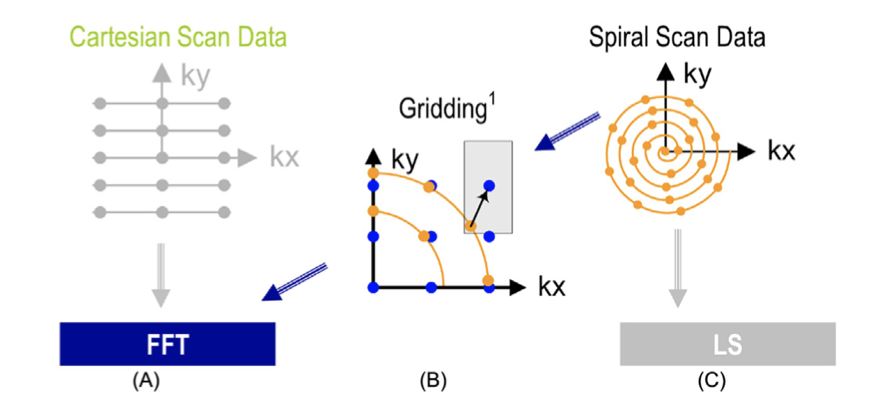
\includegraphics[width=0.9\textwidth]{figs/F17.1.png}
	\caption{\textit{扫描仪 k 空间轨迹及其相关的重建策略:(A) 采用 FFT 重建的笛卡尔轨迹,
	(B) 螺旋(或一般非笛卡尔轨迹),然后进行网格化以实现 FFT 重建,
	(C) 螺旋(非笛卡尔) 轨迹与基于线性解算器的重建。}}
\end{figure}

如果在理想条件下在 k 空间中均匀间隔的笛卡尔网格点处获取数据,则 $W(\mathbf{k})$ 加权函数是一个常数,
因此可以从等式 (17.1)的求和中分解出来。 此外,对于均匀间隔的笛卡尔网格样本,方程中的指数项。 
(17.1) 在 k 空间中均匀分布。 因此,$m(\mathbf{r})$ 的重构成为 $s(\mathbf{k})$ 上的快速傅里叶逆变换 (FFT),
这是一种极其高效的计算方法。 在这种均匀间隔的笛卡尔网格点处测量的数据集合被称为笛卡尔扫描轨迹。 
图 17.1A 描绘了笛卡尔扫描轨迹。 在实践中,笛卡尔扫描轨迹允许在扫描仪上直接实施,并且在当今的临床环境中广泛使用。

尽管笛卡尔扫描数据的逆FFT重建在计算上是高效的,
但非笛卡尔扫描轨迹通常具有降低对患者运动的敏感性、更好地提供自校准场不均匀性信息的能力以及降低对扫描仪硬件性能的要求等优点。 
因此,人们提出了非笛卡尔扫描轨迹,例如螺旋线(如图 17.1(C) 所示)、径向线(也称为投影成像)和玫瑰花结,
以减少与运动相关的伪影并解决扫描仪硬件性能限制 。 
这些改进最近使得重建的图像像素值可以用于测量微妙的现象,例如组织化学异常,然后才能成为解剖学病理学。

\begin{figure}[H]
	\centering
	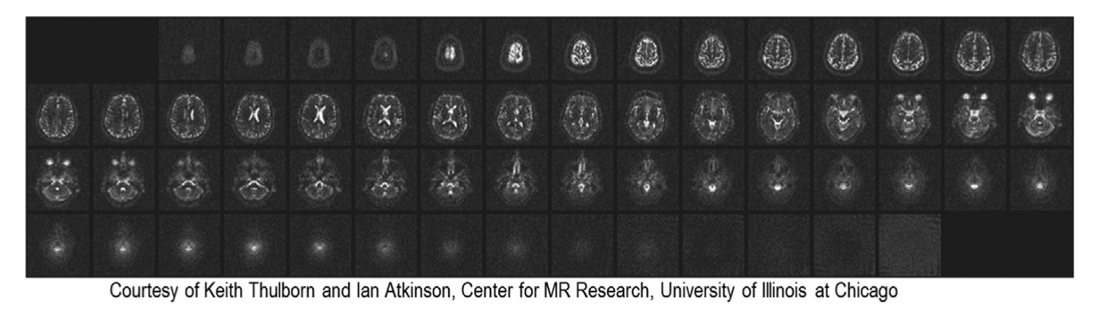
\includegraphics[width=0.9\textwidth]{figs/F17.2.png}
	\caption{\textit{非笛卡尔 k 空间样本轨迹和基于精确线性解算器的重建可实现令人兴奋的医疗应用的新功能。}}
\end{figure}

图 17.2 显示了基于 MRI 重建的测量,可生成钠图,钠是正常人体组织中受到严格监管的物质。 
该信息可用于跟踪中风和癌症治疗过程中的组织健康状况。 
由于人体组织中钠的含量远低于水分子,因此可靠地测量钠水平需要通过更多数量的样本获得更高的 SNR,
因此需要使用非笛卡尔扫描轨迹来减少额外的扫描时间。 
改进的信噪比能够可靠地收集人体组织中化学物质(例如钠)的体内浓度数据。 
钠浓度的变化或变化表明疾病发展或组织死亡的早期迹象。 
例如,图 17.2 所示的人脑钠图可用于早期指示脑肿瘤组织对化疗方案的反应,从而实现个体化医疗。

非笛卡尔轨迹数据的图像重建既带来了挑战,也带来了机遇。 主要挑战来自于指数项不再均匀分布的事实。 
求和不再具有 FFT 的形式。 因此,我们不能再通过直接对 k 空间样本应用逆 FFT 来执行重建。 
在一种称为网格化的常用方法中,首先将样本插值到均匀的笛卡尔网格上,然后使用 FFT 进行重建(见图 17.1B)。 
例如,网格化的卷积方法采用 k 空间数据点,将其与网格化卷积掩模进行卷积,并将结果累积在笛卡尔网格上。 
正如我们在第 7 章中看到的,卷积是计算密集型的,是大规模并行计算的重要模式。 
读者已经具备了通过并行计算加速卷积网格计算的技能,从而有助于将当前的 FFT 方法应用于非笛卡尔轨迹数据。

在本章中,我们将介绍一种迭代的、统计上最优的图像重建方法,该方法可以准确地模拟成像物理并限制所得图像像素值中的噪声误差。 
随着大数据分析的出现,这种统计上的最佳方法变得越来越重要。 
然而,这种迭代重建方法对于大规模三维(3D)问题来说是不切实际的,因为与网格化相比,它们的计算要求过高。 
最近,由于 GPU 的广泛可用性,这些重建在临床环境中变得可行。 
迭代重建算法过去使用高端顺序 CPU 需要花费数小时才能重建中等分辨率的图像,
现在使用 CPU 和 GPU 只需几分钟,这种延迟在临床环境中是可以接受的。

\subsection{迭代重建}
Haldar和Liang针对非笛卡尔扫描数据提出了一种基于线性求解器的迭代重建算法(Stone et al., 2008),如图17.1C所示。 该
算法允许对扫描仪数据采集过程的物理过程进行显式建模,从而减少重建图像中的伪影。 然而,它的计算成本很高。 
我们以此作为创新方法的一个例子,这些方法需要太多的计算时间才能被认为是实用的。 
我们将证明大规模并行执行可以将重建时间缩短到一分钟左右,以便可以在临床环境中部署新的成像功能(例如钠成像)。 
图 17.3 显示了基于迭代线性求解器的重建方法的拟贝叶斯估计问题公式的解决方案,
其中 $\rho$ 是包含重建图像体素值的向量,$F$ 是模拟物理场的矩阵 在成像过程中,D 是来自扫描仪的数据样本的向量,
$\mathrm{W}$ 是一个可以包含先验信息(例如解剖约束)的矩阵。 
$\mathrm{F}^{\mathrm{H}}$ 和 $\mathrm{W}^{\mathrm{H}}$ 
分别是 $\mathrm{F}$ 和 $\mathrm{W}$ 的埃尔米特转置(或共轭转置),
然后取每个条目的复共轭($a+i b$ 的复共轭为 $a-i b$ )。 
在临床环境中,$\mathrm{W}$ 中表示的解剖学约束源自对患者进行的一次或多次高分辨率、高信噪比水分子扫描。 
这些水分子扫描揭示了解剖结构位置等特征。 矩阵 $\mathrm{W}$ 是从这些参考图像导出的。 
问题是在给定所有其他矩阵和向量的情况下求解 $\rho$。

\begin{figure}[H]
	\centering
	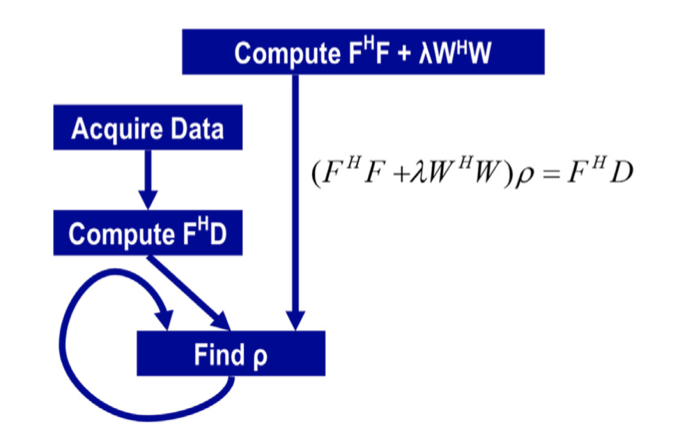
\includegraphics[width=0.9\textwidth]{figs/F17.3.png}
	\caption{\textit{一种基于迭代线性求解器的方法来重建非笛卡尔 k 空间样本数据。}}
\end{figure}

从表面上看,图 17.3 中问题表述的计算解决方案应该非常简单。 
涉及矩阵乘法和加法 $\left(\mathrm{F}^{\mathrm{H}} \mathrm{F}+\lambda \mathrm{W}^{\mathrm{H}} \mathrm{W}\right)$,
矩阵向量乘法 $\left(\mathrm{F}^{\mathrm{H}} \mathrm{D}\right)$,
矩阵求逆 $\left(\mathrm{F}^{\mathrm {H}} \mathrm{F}\right.$ $\left.+\lambda \mathrm{W}^{\mathrm{H}} \mathrm{W}\right)^{-1}$,
最后 矩阵乘法 $\left(\left(\mathrm{F}^{\mathrm{H}} \mathrm{F}+\lambda \mathrm{W}^{\mathrm{H}} \mathrm{W}\right )^{-1 *} \mathrm{~F}^{\mathrm{H}} \mathrm{D}\right)$。 
然而,矩阵的大小使得这种简单的方法极其耗时。 
$\mathrm{F}^{\mathrm{H}}$ 和 $\mathrm{F}$ 矩阵的维度由 $3 \mathrm{D}$ 重建图像中的体素数量和 重建中使用的$\mathrm{k}$ 空间样本。 
即使在适度分辨率 $128^{3}$ 体素重建中,$\mathrm{F}$ 中也有 $128^{3}=2$ 百万列,每列中有 $\mathrm{N}$ 个元素,
其中 $ \mathrm{N}$ 是使用的 $\mathrm{k}$ 空间样本的数量(D 的大小)。 显然,F 非常大。 
当人们尝试使用迭代求解器方法来估计大量噪声观测数据的主要影响因素时,在大数据分析中通常会遇到如此庞大的维度。

所涉及的矩阵的大小是如此之大,以至于使用高斯消去法等方法直接求解图 17.3 中的方程所涉及的矩阵运算实际上很棘手。 
因此,首选矩阵求逆的迭代方法,例如共轭梯度 (CG) 算法。 CG算法通过迭代求解图17.3中$\rho$的方程来重建图像。 
在每次迭代期间,CG 算法都会更新当前图像估计 $\rho$ 以提高准贝叶斯成本函数的值。 
CG技术的计算效率很大程度上取决于涉及$\mathrm{F}^{\mathrm{H}} \mathrm{F}+\lambda \mathrm{W}^{\mathrm{H}} \mathrm{W}$ 的矩阵向量乘法运算的效率和 $\rho$,
因为在 $\mathrm{CG}$ 算法的每次迭代期间都需要这些操作。

幸运的是,矩阵 $\mathrm{W}$ 通常具有稀疏结构,可以有效地实现 $\mathrm{W}^{\mathrm{H}} \mathrm{W}$,
而矩阵 $\mathrm{F }^{\mathrm{H}} \mathrm{F}$ 是 Toeplitz,它可以通过 FFT 实现高效的矩阵向量乘法。 
斯通等人。 (2008) 提出了一种用于计算 Q 的 GPU 加速方法,
这种数据结构允许我们快速计算涉及 $\mathrm{F}^{\mathrm{H}} \mathrm{F}$ 的矩阵向量乘法,
而无需实际计算 $\mathrm{F}^{\mathrm{H}} \mathrm{F}$ 本身。 
在高端 CPU 核心上,$\mathrm{Q}$ 的计算可能需要数天时间。 
由于 $\mathrm{F}$ 对图像处理的物理过程进行建模,因此对于给定的扫描仪和计划的轨迹只需执行一次。 
因此$Q$只需要计算一次,并用于使用相同扫描轨迹的多次扫描。

用于计算 $\mathrm{F}^{\mathrm{H}} \mathrm{D}$ 的矩阵向量乘法比 $\mathrm{Q}$ 大约少一个数量级,
但仍需要大约 3 小时 在高端顺序 CPU 上进行 $128^{3}$ 体素重建。 回想一下,D 是来自扫描仪的数据样本的向量。 
因此,由于每次图像采集都需要计算 $\mathrm{F}^{\mathrm{H}} \mathrm{D}$,
因此希望减少 $\mathrm{F}^{\mathrm{H}} \mathrm{D}$ 的计算时间为分钟。 
\footnote{请注意,$\mathrm{F}^{\mathrm{H}} \mathrm{D}$ 计算可以通过网格进行近似,
并且可以在几秒钟内运行,但可能会降低最终重建图像的质量。}
我们将展示此过程的详细信息。 
事实证明,$\mathrm{Q}$ 的核心计算结构与 $\mathrm{F}^{\mathrm{H}}\mathrm{D}$ 的核心计算结构相同; 
$\mathrm{Q}$ 只是涉及更多的计算,因为它处理矩阵乘法而不仅仅是矩阵向量乘法。 因此,从并行化的角度讨论其中之一就足够了。 
我们将重点关注 $\mathrm{F}^{\mathrm{H}} \mathrm{D}$,因为这是每次数据采集都需要运行的函数。

图 17.3 中的“find $\rho$”步骤根据 $\mathrm{F}^{\mathrm{H}} \mathrm{D}$ 执行实际的 CG。 
正如我们之前解释的,$\mathrm{Q}$ 的预先计算使得这一步的计算强度比 $\mathrm{F}^{\mathrm{H}} \mathrm{D}$ 少得多,
占不到 $1 \% $ 在顺序 CPU 上执行每个图像的重建。 
因此,我们将在本章中将 CG 求解器排除在并行化范围之外,并重点关注 $\mathrm{F}^{\mathrm{H}} \mathrm{D}$。 
然而,我们将在本章末尾重新审视它的状态。

\subsection{计算 $\mathbf{F}^{\mathrm{H}} \mathbf{D}$}
\begin{figure}[H]
	\centering
	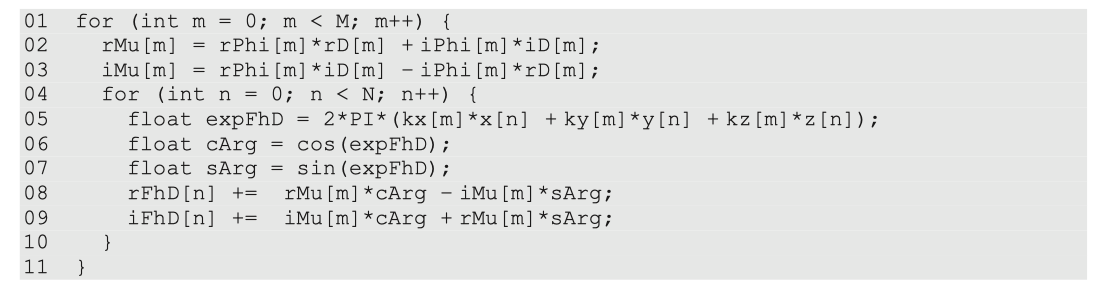
\includegraphics[width=0.9\textwidth]{figs/F17.4.png}
	\caption{\textit{$F^H D$ 的计算。}}
\end{figure}

图 17.4 显示了计算 $\mathrm{F}^{\mathrm{H}} \mathrm{D}$ 的数据结构的核心步骤的计算的顺序 $\mathrm{C}$ 实现。 
计算从迭代 k 空间样本的外循环开始(第 01 行)。 
快速浏览图 17.4 可以看出,$\mathrm{F}^{\mathrm{H}} \mathrm{D}$ 的 $\mathrm{C}$ 实现是一个很好的加速候选者,
因为它展示了大量数据 并行性。 
该算法首先计算 k 空间中当前样本点的 $\mathrm{Mu}(\mathrm{rMu}$ 和 $\mathrm{iMu}$ ) 的实部和虚部。 
然后进入一个内部 nloop,计算当前 k 空间样本对图像中每个体素 $\mathrm{F}^{\mathrm{H}} \mathrm{D}$ 实部和虚部的贡献 空间。 
请记住,$\mathrm{M}$ 是$\mathrm{k}$ 空间样本的总数,$\mathrm{N}$ 是重建图像中体素的总数。 
任意体素处的 $\mathrm{F}^{\mathrm{H}} \mathrm{D}$ 的值取决于所有 $\mathrm{k}$ 空间样本点的值。 
然而,$\mathrm{F}^{\mathrm{H}} \mathrm{D}$ 的体素元素不依赖于 
$\mathrm{F}^{\mathrm{H}} \mathrm{D}$ 的任何其他体素元素。 
因此 $\mathrm{F}^{\mathrm{H}} \mathrm{D}$ 的所有元素都可以并行计算。 
具体地,外循环的所有迭代可以并行完成,并且内循环的所有迭代可以并行完成。 
然而,内循环的计算依赖于外循环的同一迭代中前面的语句所完成的计算。

尽管该算法具有丰富的固有并行性,但潜在的性能瓶颈是显而易见的。 
首先,在计算 $\mathrm{F}^{\mathrm{H}} \mathrm{D}$ 元素的循环中,
浮点运算与内存访问的比率最多为 $0.75 \mathrm{OP} / \mathrm{B}$,最差 $0.25 \mathrm{OP} / \mathrm{B}$。 
最好的情况假设 sin 和 cos 三角运算是通过使用分别需要 13 次和 12 次浮点运算的五元素泰勒级数来计算的。 
最坏的情况假设每个三角运算都作为硬件中的单个运算进行计算。 
正如我们在第 5 章“内存架构和数据局部性”中看到的,为了使内核不受内存带宽的限制,需要更高的浮点运算与全局内存访问比率。 
因此,除非大幅增加比率,否则内存访问将明显限制内核的性能。

其次,浮点算术与浮点三角函数的比例仅为13:2。 
因此,基于 GPU 的实现必须容忍或避免由于正弦和余弦运算的长延迟和低吞吐量而导致的停顿。 
如果没有好的方法来降低三角函数的成本,性能可能会受到这些函数所花费的时间的支配。 
我们现在准备采取步骤将 $\mathrm{F}^{\mathrm{H}} \mathrm{D}$ 从连续的 $\mathrm{C}$ 代码转换为 CUDA 内核。

\subsubsection{第 1 步:确定内核并行结构}
\begin{figure}[H]
	\centering
	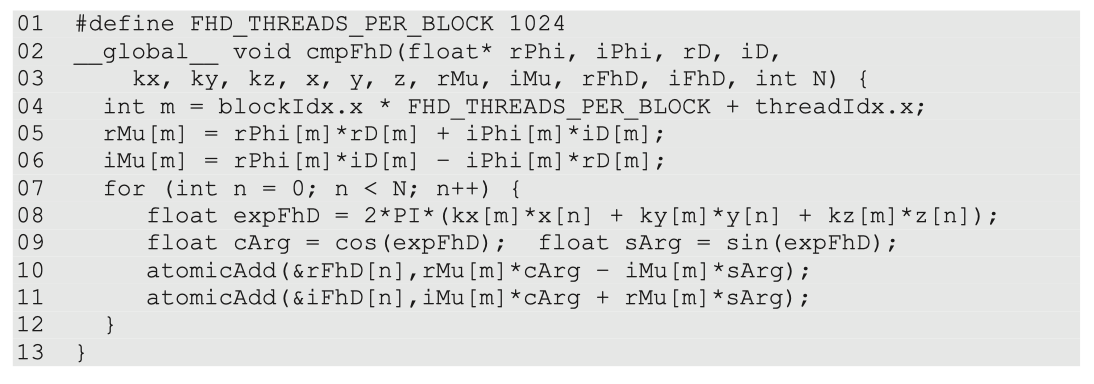
\includegraphics[width=0.9\textwidth]{figs/F17.5.png}
	\caption{\textit{$F^H D$ 内核的第一个版本。}}
\end{figure}

将图 17.4 中的循环转换为 CUDA 内核在概念上很简单。 
由于图 17.4 的外循环的所有迭代都可以并行执行,因此我们可以通过将其迭代映射到 CUDA 线程来简单地将外循环转换为 CUDA 内核。 
图 17.5 显示了来自这种简单转换的内核。 每个线程实现原始外循环的迭代; 
也就是说,我们使用每个线程来计算一个 k 空间样本对所有 $\mathrm{F}^{\mathrm{H}} \mathrm{D}$ 元素的贡献。 
原始外循环有 $\mathrm{M}$ 次迭代,$\mathrm{M}$ 可能有数百万次。 
显然,我们需要有大量的线程块来生成足够的线程来实现所有这些迭代。

为了使性能调整变得容易,我们声明一个常量 FHD\_THREADS\_PER\_BLOCK ,
它定义了当我们调用 $\mathrm{cmpFhD}$ 内核时每个线程块中的线程数。 
因此,在调用内核时,我们将使用 M/ FHD\_THREADS\_PER\_BLOCK 作为网格大小,
使用 FHD\_THREADS\_PER\_BLOCK 作为块大小。 
在内核中,每个线程使用熟悉的公式 blockIdx 计算分配给它覆盖的外部循环的原始迭代。 
$x^{*} F$ HD\_THREADS\_PER\_BLOCK + threadIdx.x。 
例如,假设有 1,000,000 个 k 空间样本,并且我们决定每个块使用 1024 个线程。 
内核创新时的网格大小将为 1,000,000/1024=977 个区块。 块大小将为 1,024 。 
每个线程的$\mathrm{m}$的计算将相当于blockIdx.x * 1024+threadIdx.

虽然图 17.5 的内核利用了充足的并行性,但它遇到了一个主要问题:所有线程都写入所有 $\mathrm{rFhD}$ 
和 $\mathrm{iFhD}$ 体素元素。 
这意味着内核必须在内循环中的全局内存中使用原子操作,以防止线程破坏彼此对体素值的贡献(第 10-11 行)。 
正如我们在第 9 章“平行直方图”中看到的,重
对全局内存数据使用原子操作会严重降低并行执行的性能。 
此外,$\mathrm{rFhD}$和$\mathrm{iFhD}$数组的大小(重建图像中体素的总数)使得共享内存中的私有化不可行。 
我们需要探索其他选择。

每个线程获取输入元素(本应用中的 k 空间样本)并更新所有或多个输出元素(本应用中的重建图像的体素)的安排被称为分散方法。 
直观上,每个线程将输入的效果分散到许多输出值。 不幸的是,分散方法中的线程可以更新相同的输出元素,并可能破坏彼此的贡献。 
因此,原子操作通常是分散方法所必需的,并且往往会对并行执行的性能产生负面影响。

分散方法的一种可能更好的替代方法是使用每个线程通过收集所有输入元素的贡献来计算一个输出元素,这称为聚集方法。 
收集方法可确保线程仅更新其指定的输出元素,并且不会相互干扰。 
在我们的应用程序中,基于聚集方法的并行化分配每个线程从所有 $\mathrm{k}$ 空间样本中计算一对 $\mathrm{rFhD}$ 
和 $\mathrm{iFhD}$ 元素。 这样一来,线程之间就没有干扰,也不需要原子操作。

为了采用聚集方法,我们需要将 n 循环作为外循环,以便我们可以将 n 循环的每次迭代分配给一个线程。 
这可以通过交换图 17.4 中的内循环和外循环来完成,
以便每个新的外循环迭代处理一个 $\mathrm{rFhD} / \mathrm{iFhD}$ 元素对。 
也就是说,每次新的外循环迭代将执行新的内循环,
该循环累积所有 $\mathrm{k}$ 空间样本对处理的 $\mathrm{rFhD} / \mathrm{iFhD}$ 元素对的贡献 通过外循环迭代。 
循环结构的这种变换称为循环交换。 
它需要一个完美的嵌套循环,这意味着外部 for 循环语句和内部 for 循环语句之间没有任何语句。 
然而,对于图 17.4 中的 FhD 代码来说,情况并非如此。 我们需要找到一种方法来移动 rMu 和 iMu 元素的计算。

\begin{figure}[H]
	\centering
	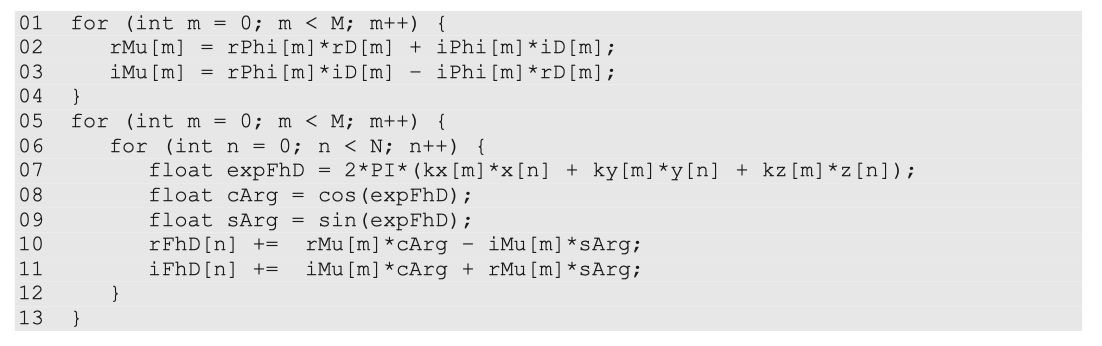
\includegraphics[width=0.9\textwidth]{figs/F17.6.png}
	\caption{\textit{$F^H D$ 计算上的循环裂变。}}
\end{figure}

通过快速检查图 17.4,我们可以看到 $\mathrm{F}^{\mathrm{H}} \mathrm{D}$ 计算可以分为两个单独的循环,
如图 17.6 所示,使用 一种称为循环裂变或循环分裂的技术。 
此转换采用循环体并将其分成两个循环。 对于$\mathrm{F}^{\mathrm{H}} \mathrm{D}$,
外循环由两部分组成:内循环之前的语句和内循环本身。 
如图17.6所示,我们可以将内循环之前的语句放入第一个循环,将内循环放入第二个循环,从而对外循环进行循环裂变。

循环裂变中的一个重要考虑因素是转换改变了原始外循环两部分的相对执行顺序。 
在原始外循环中,第一次迭代的两个部分都在第二次迭代之前执行。 
裂变之后,所有迭代的第一部分将执行; 然后是所有迭代的第二部分。 
读者应该能够验证执行顺序的更改不会影响 $\mathrm{F}^{\mathrm{H}} \mathrm{D}$ 的执行结果。 
这是因为每次迭代的第一部分的执行不依赖于原始外循环的任何先前迭代的第二部分的结果。 
循环裂变是一种通常由高级编译器完成的转换,这些编译器能够分析跨循环迭代的语句之间的(缺乏)依赖性。

通过循环裂变,$\mathrm{F}^{\mathrm{H}} \mathrm{D}$ 计算现在分两步完成。 
第一步是单级循环,计算第二个循环中使用的 $\mathrm{rMu}$ 和 $\mathrm{iMu}$ 元素。 
第二步对应于第二个循环,根据 $\mathrm{rMu}$ 和 $\mathrm{iMu}$ 
计算 $\mathrm{F}^{\mathrm{H}} \mathrm{D}$ 元素 第一步计算出的元素。 现在每个步骤都可以转换为自己的 CUDA 内核。 
两个 CUDA 内核将彼此顺序执行。 
由于第二个循环需要使用第一个循环的结果,因此将这两个循环分成两个按顺序执行的内核不会牺牲任何并行性。

\begin{figure}[H]
	\centering
	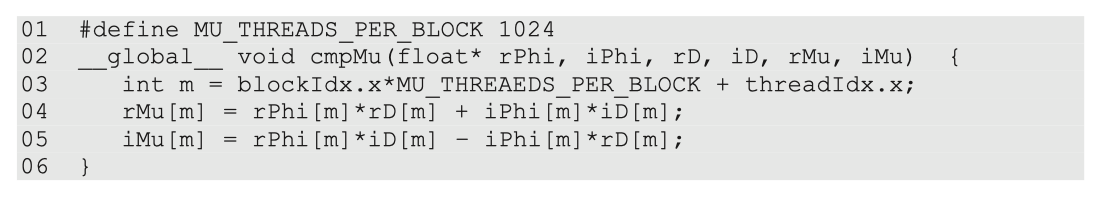
\includegraphics[width=0.9\textwidth]{figs/F17.7.png}
	\caption{\textit{cmpMu 内核。}}
\end{figure}

图 17.7 中的 cmpMu() 内核实现了第一个循环。 
第一个循环从连续的 $\mathrm{C}$ 代码到 CUDA 内核的转换非常简单:每个线程执行原始 $C$ 代码的一次迭代。 
由于$M$值可能非常大,反映了大量的k空间样本,因此这种映射可能会导致大量的线程。 
由于每个线程块最多可以有 1024 个线程,因此我们需要使用多个块来允许大量线程。 
这可以通过在每个块中拥有多个线程(由图 17.7 中的 MU\_THREADS\_PER\_BLOCK 指定)
并使用覆盖原始循环的所有 M 次迭代所需的 M/MU\_THREADS\_PER\_BLOCK 块来实现。
例如,如果有 1,000,000 个 k 空间样本,则可以使用每个块 1024 个线程和 $1,000,000 / 1024=977$ 块的配置来调用内核。 
这是通过在内核创新期间将 MU\_THREADS\_PER\_BLOCK 定义为 1024 
并将其用作块大小和 M/MU\_THREADS\_PER\_BLOCK 作为网格大小来完成的。

在内核中,每个线程都可以使用其 blockIdx 和 threadIdx 值来识别分配给它的迭代。 
由于线程结构是一维的,因此只需要使用blockIdx.x和threadIdx.x。 
由于每个块覆盖原始迭代的一部分,因此线程覆盖的迭代为 blockIdx.x *MU\_THREADS\_PER\_BLOCK + threadIdx。 
例如,假设 MU\_THREADS\_PER\_BLOCK $=1024$。 具有 blockIdx 的线程。 $x=0$ 和 threadIdx。 
$x=37$ 覆盖原始循环的第 37 次迭代,而带有 blockIdx 的线程。 $x=5$ 和 threadIdx。 
$x=2$ 覆盖原始循环的第 5122 次 $\left(5^{*} 1024+2\right)$ 迭代。 
使用此迭代编号访问 $\mathrm{Mu}$、Phi 和 D 数组可确保线程覆盖数组的方式与原始循环迭代覆盖数组的方式相同。 
因为每个线程都写入自己的 $\mathrm{Mu}$ 元素,所以这些线程之间不存在潜在的冲突。

确定第二个内核的结构需要做更多的工作。 对图 17.6 中第二个循环的检查表明,设计第二个内核时至少有三个选项。 
在第一个选项中,每个线程对应于内部循环的一次迭代。 此选项创建最多数量的线程,从而利用最大数量的并行性。 
但是,线程数量为 $\mathrm{N}^{*} \mathrm{M}$,其中 $\mathrm{N}$ 为数百万,$\mathrm{M}$ 为数十万。 
他们的产品会导致网格中的线程过多,超出了充分利用该设备所需的数量。

第二种选择是使用每个线程来实现外循环的迭代。 此选项比第一个选项使用更少的线程。 
该选项不是生成 $\mathrm{N}^{*} \mathrm{M}$ 线程,而是生成 $\mathrm{M}$ 线程。 
由于 $\mathrm{M}$ 对应于 k 空间样本的数量,
并且通常使用十万数量级的大量样本来计算 $\mathrm{F}^{\mathrm{H} } \mathrm{D}$,这个选项仍然利用了大量的并行性。 
然而,这个内核遇到了与图 17.5 中的内核相同的问题。 
也就是说,每个线程都会写入所有$\mathrm{rFhD}$和$\mathrm{iFhD}$元素,从而在线程之间产生极大量的冲突。 
与图 17.5 的情况一样,图 17.8 中的代码需要原子操作,这将显着减慢并行执行速度。 因此这个选项效果不佳。

\begin{figure}[H]
	\centering
	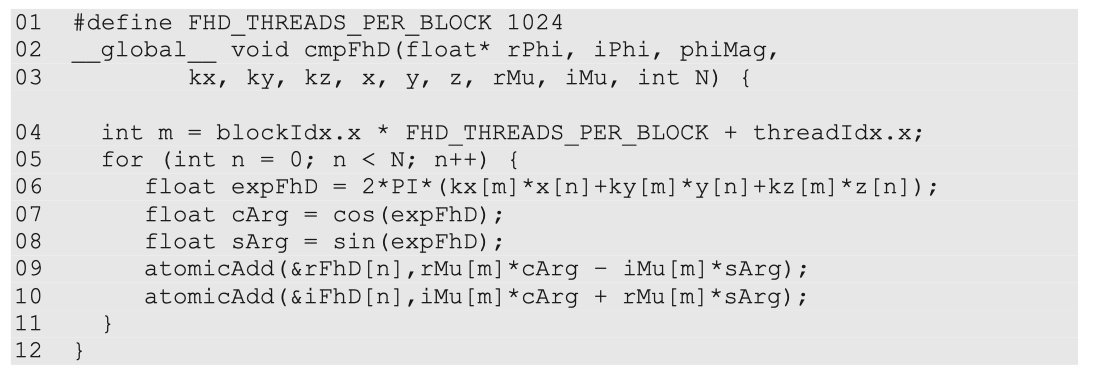
\includegraphics[width=0.9\textwidth]{figs/F17.8.png}
	\caption{\textit{$F^H D$ 内核的第二个选择。}}
\end{figure}

\begin{figure}[H]
	\centering
	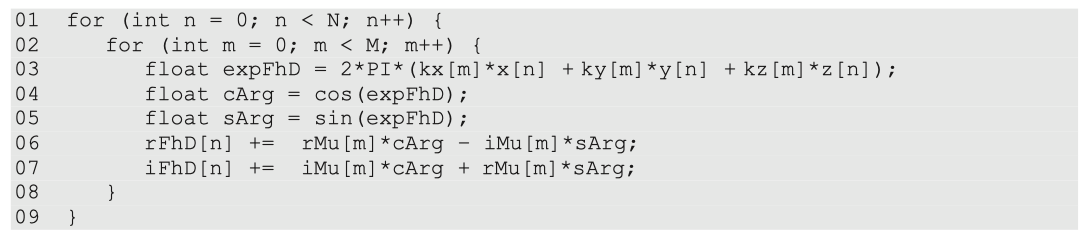
\includegraphics[width=0.9\textwidth]{figs/F17.9.png}
	\caption{\textit{$F^H D$ 计算的循环交换。}}
\end{figure}

第三种选择是使用每个线程计算一对 $\mathrm{rFhD}$ 和 $\mathrm{iFhD}$ 输出元素。 
此选项要求我们互换内循环和外循环,然后使用每个线程来实现新外循环的迭代。 
变换如图 17.9 所示。 循环交换是必要的,因为 CUDA 线程实现的循环必须是外循环。 
循环交换使每个新的外循环迭代处理一对 $\mathrm{rFhD}$ 和 $\mathrm{iFhD}$ 输出元素,
并使每个内循环收集所有输入元素对这对输出元素的贡献。

这里允许循环互换,因为两级循环的所有迭代都是彼此独立的。 它们可以以任何相对于彼此的顺序执行。 
当这些迭代可以以任何顺序执行时,允许改变迭代顺序的循环交换。 该选项允许我们将新的外循环转换为由 N 个线程执行的内核。 
由于 N 对应于重建图像中的体素数量,因此对于更高分辨率的图像,$\mathrm{N}$ 值可能非常大。 
对于$128^{3}$的图像,有$128^{3}=$$2,097,152$个线程,导致大量的并行。 
对于更高分辨率,例如 $512^{3}$,我们可能需要使用多维网格、启动多个网格或将多个体素分配给单个线程。 
第三个选项中的线程都累积到自己的 $\mathrm{rFhD}$ 和 $\mathrm{iFhD}$ 元素中,
因为每个线程都有唯一的 $\mathrm{n}$ 值。 线程之间不存在冲突。 这使得第三个选项成为三个选项中的最佳选择。

\begin{figure}[H]
	\centering
	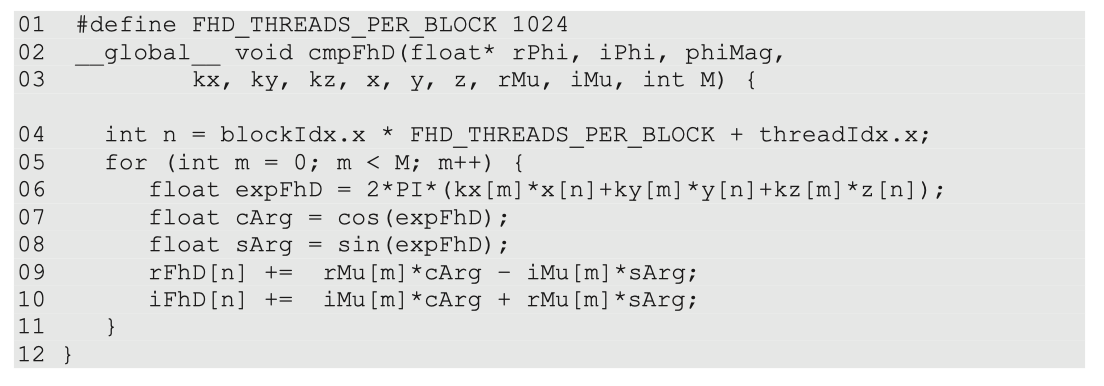
\includegraphics[width=0.9\textwidth]{figs/F17.10.png}
	\caption{\textit{$F^H D$ 内核的第三个选择。}}
\end{figure}

从交换循环中导出的内核如图 17.10 所示。 
外环已被剥离; 每个线程覆盖外层 (n) 循环的迭代,
其中 $\mathrm{n}$ 等于 blockIdx.x*FH\_THREADS\_PER\_BLOCK + threadIdx.x。 
一旦确定了迭代 (n) 值,线程就会根据该 $\mathrm{n}$ 值执行内部 (m) 循环。 
该内核可以通过每个块中的多个线程来调用,这些线程由全局常量 FHD\_THREADS\_PER\_BLOCK 指定。 
假设 $\mathrm{N}$ 是存储重建图像中体素数量的变量,则 N/FHD\_THREADS\_PER\_BLOCK 块覆盖原始循环的所有 N 次迭代。 
例如,如果有 2,097,152 个体素,则可以使用每块 1024 个线程和 2,097,152/1024 = 2048 个块的配置来调用内核。 
在图 17.10 中,这是通过在内核调用期间将 1024 分配给 FHD\_THREADS\_PER\_BLOCK 
并将其用作块大小和 N/FHD\_THREADS\_PER\_BLOCK 作为网格大小来完成的。

\subsubsection{第 2 步:绕过内存带宽限制}
图 17.10 中的简单 cmpFhD 内核的性能明显优于图 17.10 和图 17.10 中的内核。 
17.5 和 17.8,但由于内存带宽限制,加速仍然有限。 快速分析表明,执行受到每个线程的低计算与全局内存访问比率的限制。 
在原始循环中,每次迭代至少执行 14 次内存访问: $k x[m], k y[m], k z$ $[m], x[n], y[n], z[n], r M u [m]$ 两次,
$i M u[m]$ 两次,$r F h D[n]$ 读写,$\mathrm{iFhD}[\mathrm{n}]$ 读写。 
同时,每次迭代中执行约 13 次浮点乘法、加法或三角运算。 
因此,计算与全局内存访问的比率为 $13 /\left(14^{*} 4\right)=0.23 \mathrm{OP} / \mathrm{B}$,
根据我们在第 5 章中的分析,这个比率太低了, 内存架构和数据局部性。 
通过将一些数组元素分配给自动变量,我们可以立即提高计算与全局内存访问的比率。 
正如我们在第 5 章“内存架构和数据局部性”中讨论的那样,自动变量将驻留在寄存器中,
从而将对全局内存的读取和写入转换为对片上寄存器的读取和写入。 
快速回顾图 17.10 中的内核表明,
对于每个线程,在 for 循环的所有迭代中都使用相同的 $x[n]、y[n]$ 和 $z[n]$ 元素(行 05-06)。 
这意味着我们可以在执行进入循环之前将这些元素加载到自动变量中。 
然后,内核可以在循环内使用自动变量,从而将全局内存访问转换为寄存器访问。 
此外,循环重复读取和写入$\mathrm{rFhD}[\mathrm{n}]$和$\mathrm{iFhD}[\mathrm{n}]$。 
我们可以让迭代读取和写入两个自动变量,
并仅将这些自动变量的内容写入 $\mathrm{rFhD}[\mathrm{n}]$ 和 $\mathrm{iFhD}[\mathrm{n} ]$ 执行后退出循环。 
生成的代码如图 17.11 所示。 通过将每个线程使用的寄存器数量增加 5 个,我们将每次迭代中完成的内存访问从 14 次减少到 7 次。 
因此,我们将计算与全局内存访问的比率从 $0.23 \mathrm{OP} / \mathrm{B}$ 增加到 $0.46 \mathrm{OP} / \mathrm{B}$。 
这是一个很好的改进,也很好地利用了宝贵的寄存器资源。

回想一下,寄存器的使用可以限制占用率,即流式多处理器(SM)中可以运行的块的数量。 
通过在内核代码中将寄存器使用量增加 5,我们将每个线程块的寄存器使用量增加了 5*FHD\_THREADS\_PER\_BLOCK。 
假设每个块有 1024 个线程,我们只是将块寄存器使用量增加了 5120 个。
由于每个 SM 可以在分配给它的所有块中容纳 65,536 个寄存器的组合寄存器使用量(在 SM 版本 3.5 或更高版本中),
因此我们需要 请小心,因为寄存器使用量的任何进一步增加都可能开始限制可分配给 SM 的块数量。 
幸运的是,寄存器的使用并不是该内核并行性的限制因素。

\begin{figure}[H]
	\centering
	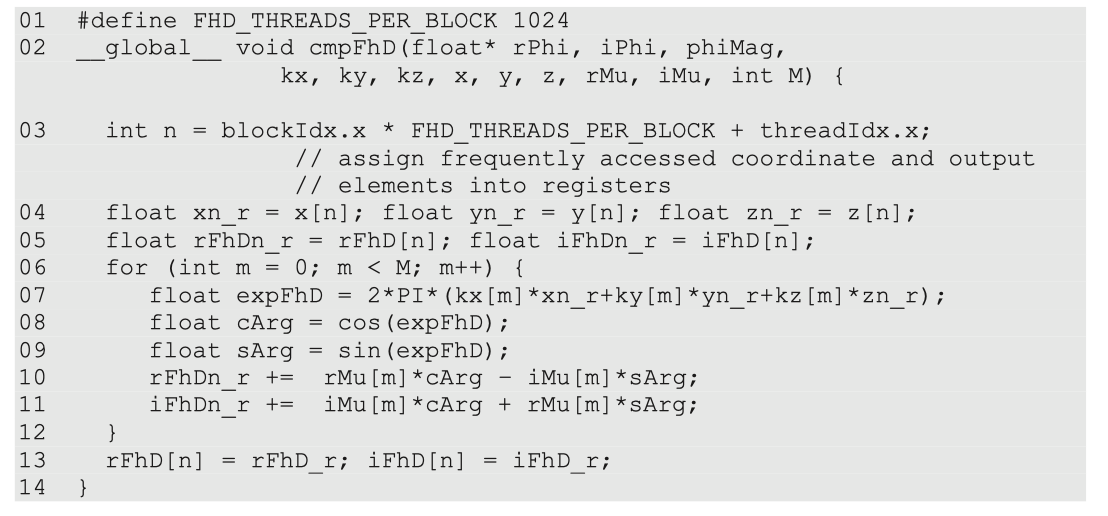
\includegraphics[width=0.9\textwidth]{figs/F17.11.png}
	\caption{\textit{使用寄存器来减少 $F^H D$ 内核中的内存访问。}}
\end{figure}

我们希望通过消除 cmpFhD 内核中更多的全局内存访问来进一步提高计算与全局内存访问的比率。 
接下来要考虑的候选是 $\mathrm{k}$ 空间样本 $\mathrm{kx}[\mathrm{m}]、\mathrm{ky}[\mathrm{m}]$ 
和 $\mathrm{ kz}[\mathrm{m}]$。 这些数组元素的访问方式与 $x[n]、y[n]$ 和 $z[n]$ 元素不同:
在图 17.11 中的循环的每次迭代中访问 kx、ky 和 kz 的不同元素 。 
这意味着我们无法将 k 空间元素加载到寄存器中并期望通过所有迭代从寄存器中访问该元素。 因此寄存器在这里没有帮助。 
但是,我们应该注意到 k 空间元素不会被内核修改。 此外,每个 k 空间元素都在网格中的所有线程中使用。 
这意味着我们可以将 k 空间元素放入常量内存中。 也许恒定的高速缓存可以消除大部分 DRAM 访问。 
对图 17.11 中循环的分析表明,k 空间元素确实是常量存储器的绝佳候选者。 
用于访问$\mathrm{kx}、\mathrm{ky}$和$\mathrm{kz}$的索引是$\mathrm{m}$。 
我们知道 $\mathrm{m}$ 独立于 threadIdx,这意味着 warp 中的所有线程都将访问 kx、ky 和 kz 的相同元素。 
这是缓存常量内存的理想访问模式:每次将一个元素放入缓存时,它至少会被当前一代设备的 warp 中的所有 32 个线程使用。 
这意味着对于常量内存的每 32 次访问,缓存将至少服务其中 31 次。 这使得缓存能够有效地消除 $96 \%$ 或更多对全局内存的访问。 
更好的是,每次从缓存访问常量时,都可以将其广播到warp中的所有线程。 
这使得常量内存几乎与访问 $\mathrm{k}$ 空间元素的寄存器一样高效。
\footnote{常量存储器访问并不完全像寄存器访问那样有效的原因是,访问常量存储器仍然需要存储器加载指令。}

然而,将 k 空间元素放入常量存储器中涉及一个技术问题。 回想一下,常量内存的容量为 $64 \mathrm{~KB}$。 
然而,k 空间样本的大小可能要大得多,达到数百万的数量级。 
解决恒定内存容量限制的典型方法是将大型数据集分解为 64 $\mathrm{~KB}$ 或更小的块。 
开发人员必须重新组织内核,以便多次调用内核,每次调用内核仅消耗大数据集的一部分。 
这对于 $\mathrm{cmpFhD}$ 内核来说非常容易。

仔细检查图 17.11 中的循环表明,所有线程都将按顺序遍历 k 空间样本数组。 
也就是说,网格中的所有线程在每次迭代期间都访问相同的 k 空间元素。 对于大型数据集,内核中的循环只是迭代更多次。 
这意味着我们可以将循环分为几个部分,每个部分处理适合 $64 \mathrm{~KB}$ 常量内存容量的 k 空间元素块。 
\footnote{请注意,并非所有对只读数据的访问都像我们这里的那样有利于常量内存。 
在某些应用程序中,不同块中的线程在同一迭代中访问不同的输入元素。 
这种更加分散的访问模式使得将足够的数据放入常量内存以供内核启动变得更加困难。}
主机代码现在多次调用内核。 每次主机调用内核时,它都会在调用内核函数之前将一个新块放入常量内存中。 
如图 17.12 所示。 (对于更新的设备和 CUDA 版本,
内核参数的“const\_restrict\_”声明使相应的输入数据在只读数据缓存中可用,这是获得与使用常量内存相同效果的更简单方法。 )

\begin{figure}[H]
	\centering
	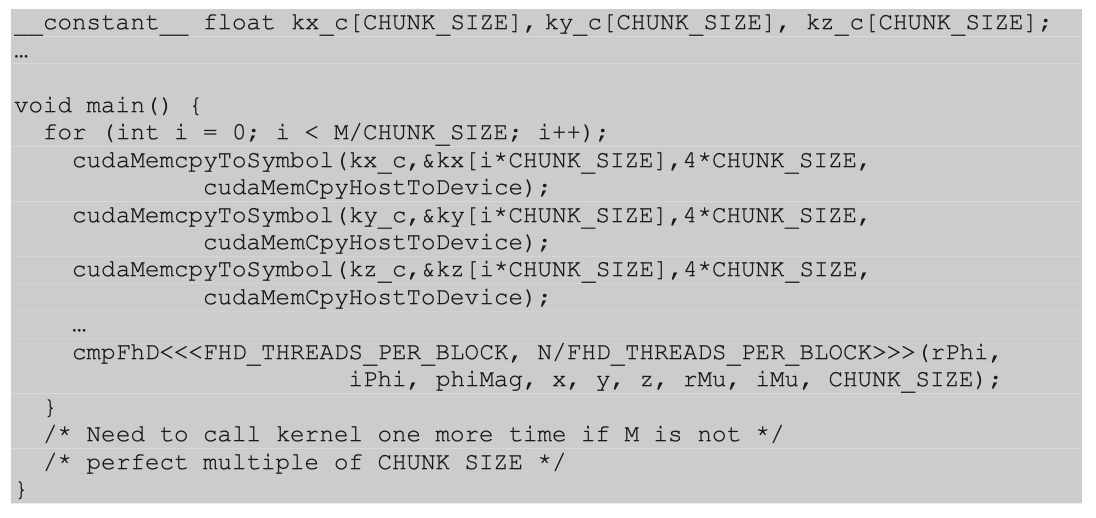
\includegraphics[width=0.9\textwidth]{figs/F17.12.png}
	\caption{\textit{用于对 k 空间数据进行分块以适合常量内存的主机代码序列。}}
\end{figure}

在图 17.12 中,cmpFhD 内核是从循环中调用的。 
该代码假设 $\mathrm{kx}、\mathrm{ky}$ 和 $\mathrm{kz}$ 数组位于主机内存中。 
$\mathrm{kx}、\mathrm{ky}$ 和 $\mathrm{kz}$ 的维度由 M 给出。
在每次迭代中,主机代码调用 cudaMemcpyToSymbol ( ) 函数来传输 k- 的块 将数据空间数据放入设备常量内存中,
如第 7 章卷积中所讨论的,然后调用内核来处理该块。 
请注意,当 $M$ 不是 CHUNK\_SIZE 的完美倍数时,
主机代码将需要额外一轮 cudaMemcpyToSymbol() 和一次内核调用来完成剩余的 k 空间数据。

\begin{figure}[H]
	\centering
	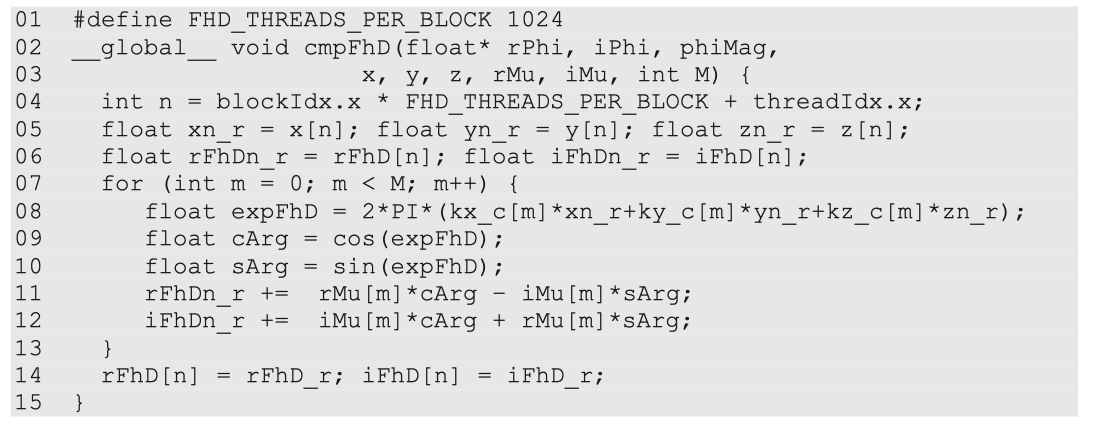
\includegraphics[width=0.9\textwidth]{figs/F17.13.png}
	\caption{\textit{修改了 $F^H D$ 内核以使用常量内存。}}
\end{figure}

图 17.13 显示了一个修改后的内核,它从常量存储器访问 k 空间数据。 
请注意,指向 $\mathrm{kx}$、ky 和 $\mathrm{kz}$ 的指针不再出现在核函数的参数列表中。 
kx\_c、ky\_c 和 kz\_c 数组作为在 \_\_constant\_ 关键字下声明的全局变量来访问,如图 17.12 所示。 
通过从常量高速缓存访问这些元素,内核现在实际上只有四次对 rMu 和 iMu 数组的全局内存访问。 
编译器通常会识别出四个数组访问仅针对两个位置。 
它将仅执行两次全局访问,一次访问 $\mathrm{rMu}[\mathrm{m}]$,一次访问 $i \mathrm{Mu}[\mathrm{m}]$。 
这些值将存储在临时寄存器变量中,以供其他两个变量使用。 这使得最终的内存访问次数等于 2 。 
计算与内存访问比率高达 $1.63 \mathrm{OP} / \mathrm{B}$。 
这仍然不太理想,但足够高,内存带宽限制不再是限制性能的唯一因素。 
正如我们将看到的,我们可以执行一些其他优化,使计算更加高效并进一步提高性能。

\begin{figure}[H]
	\centering
	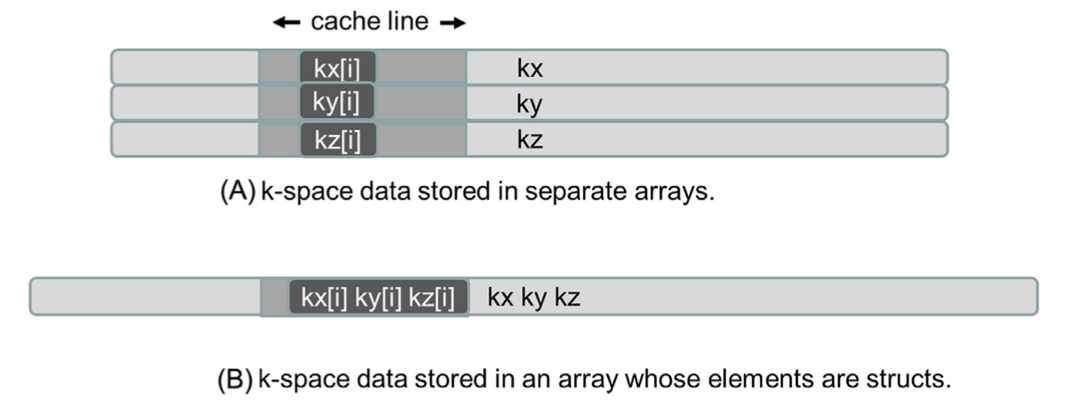
\includegraphics[width=0.9\textwidth]{figs/F17.14.png}
	\caption{\textit{k 空间数据布局对恒定缓存效率的影响:(A) k 空间数据存储在单独的数组中,
	(B) k 空间数据存储在其元素为结构的数组中。}}
\end{figure}

如果我们运行图中的代码。 在 17.12 和 17.13 中,我们会发现某些设备的性能增强并没有我们预期的那么高。 
事实证明,这些图中显示的代码并没有像我们预期的那样减少内存带宽。 原因是常量缓存对于代码来说表现不佳。 
这与常量缓存的设计和k空间数据的内存布局有关。 如图17.14A所示,每个常量高速缓存条目被设计为存储多个连续的字。 
这种设计降低了恒定缓存硬件的成本。 当一个元素被放入缓存时,它周围的几个元素也会被放入缓存。 
这被说明为围绕 $\mathrm{kx}$ [i]、ky[i] 和 kz[i] 的阴影部分,在图 17.14 中显示为黑框。 
常量高速缓存中需要三个高速缓存行来支持warp的每次迭代的高效执行。

在典型的执行中,我们将有相当大量的 warp 在 SM 上同时执行。 
由于不同的warp可能处于非常不同的迭代,因此它们可能需要许多恒定的缓存条目。 
例如,如果我们将每个线程块定义为具有 1024 个线程,并期望分配两个块在每个 SM 中并发执行,
则我们将在 SM 中同时执行 (1024/ $32) \times 2=64$ 个warp。 
如果它们中的每一个都需要常量缓存中至少三个缓存行来维持高效执行,那么在最坏的情况下,
我们总共需要 $64 \times 3=192$ 缓存行。 
即使我们假设平均而言,三个 warp 将在同一迭代中执行,从而可以共享缓存行,我们仍然需要 64 个缓存行。 
这称为所有活动warp的工作集。

由于成本限制,一些设备的constant cache的cache line数量较少,比如32条。 
当没有足够的缓存行来容纳整个工作集时,不同warp访问的数据开始相互竞争缓存行。 
当warp移动到下一个迭代时,下一个要访问的元素已经被清除,以便为其他warp已访问的元素腾出空间。 
事实证明,某些设备中的恒定缓存容量确实不足以容纳 SM 中所有活动的 warp 的条目。 
因此,常量高速缓存无法消除许多全局内存访问。

\begin{figure}[H]
	\centering
	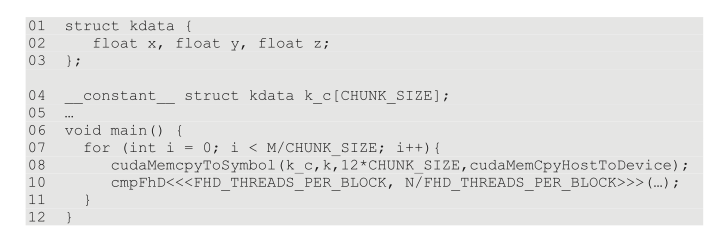
\includegraphics[width=0.9\textwidth]{figs/F17.15.png}
	\caption{\textit{调整k空间数据布局,提高缓存效率。}}
\end{figure}

\begin{figure}[H]
	\centering
	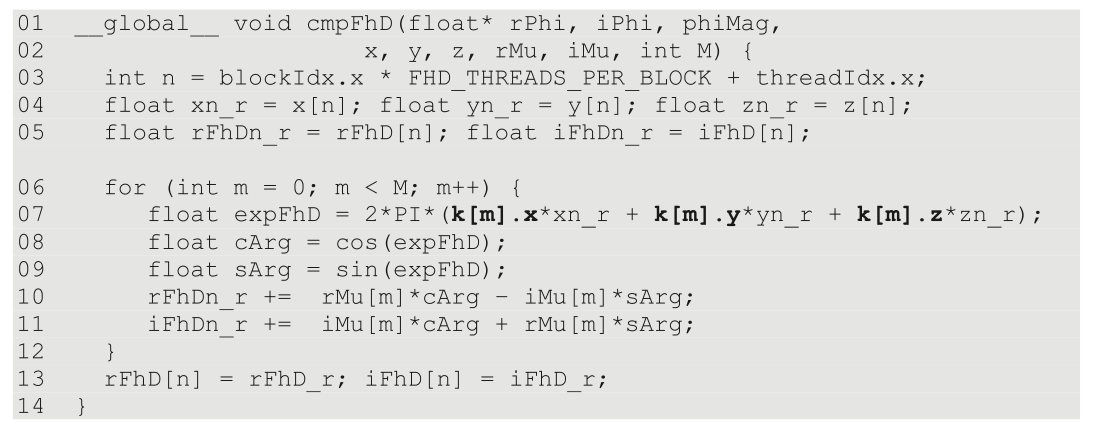
\includegraphics[width=0.9\textwidth]{figs/F17.16.png}
	\caption{\textit{调整 $F^H D$ 内核中的 k 空间数据内存布局。}}
\end{figure}

缓存条目使用效率低下的问题在文献中已经得到了很好的研究,并且可以通过调整k空间数据的内存布局来解决。 
该方案如图17.14B所示,基于该方案的代码如图  17.15 和 17.16 所示。 
该解决方案不是将 k 空间数据的 $\mathrm{x}、\mathrm{y}$ 和 $\mathrm{z}$ 分量存储在三个单独的数组中,
而是将这些分量存储在一个数组中,该数组的元素使 建立一个结构体。 在文献中,这种声明方式通常称为结构数组。 
数组的声明如图 17.15(第 01-03 行)所示。 
我们假设内存分配和初始化代码(未显示)已将 $\mathrm{x}、\mathrm{y}$ 和 $\mathrm{z}$ 组件
放置在 $\mathrm{k}$ 空间中 数据正确输入字段。 
通过将 $\mathrm{x}、\mathrm{y}$ 和 $\mathrm{z}$ 分量存储在数组元素的三个字段中,
开发人员强制将这些分量存储在常量内存的连续位置中 。 
因此,warp 迭代使用的所有三个组件现在都可以放入一个缓存条目中,从而减少支持所有活动 warp 执行所需的条目数量。 
请注意,由于我们只有一个数组来保存所有 k 空间数据,
因此我们可以仅使用一个 CUDA Memcpy To Symbol 将整个块复制到设备常量内存。 
假设每个k空间样本都是单精度浮点数,
则传输的大小从$4{}^{*}$CHUNK\_SIZE调整为$12^{*}$CHUNK\_SIZE
以反映传输 一个 CUDA Memcpy To Symbol 调用中的所有三个组件。

使用新的数据结构布局,我们还需要修改内核,以便根据新的布局进行访问。 新内核如图 17.16 所示。 
请注意, $\mathrm{kx}[\mathrm{m}]$ 已变为 $\mathrm{k}[\mathrm{m}].\mathrm{x}, \mathrm{ky}[\mathrm{m}]$ 已变为 $\mathrm{k}[\mathrm{m}].\mathrm{y}$ 等等。 
对代码的这一小改动可以显着提高其在某些设备上的执行速度。
\footnote{读者可能会注意到,从多个数组到结构数组的调整与通常对全局内存数据所做的操作相反。 
当 warp 中的相邻线程访问全局内存中结构数组的连续元素时,最好将该结构的字段存储到多个数组中,以便合并全局内存访问。 
这里的关键区别在于,warp 中的所有线程都访问相同的元素,而不是连续的元素。}

\subsubsection{第 3 步:使用硬件三角函数}
\begin{figure}[H]
	\centering
	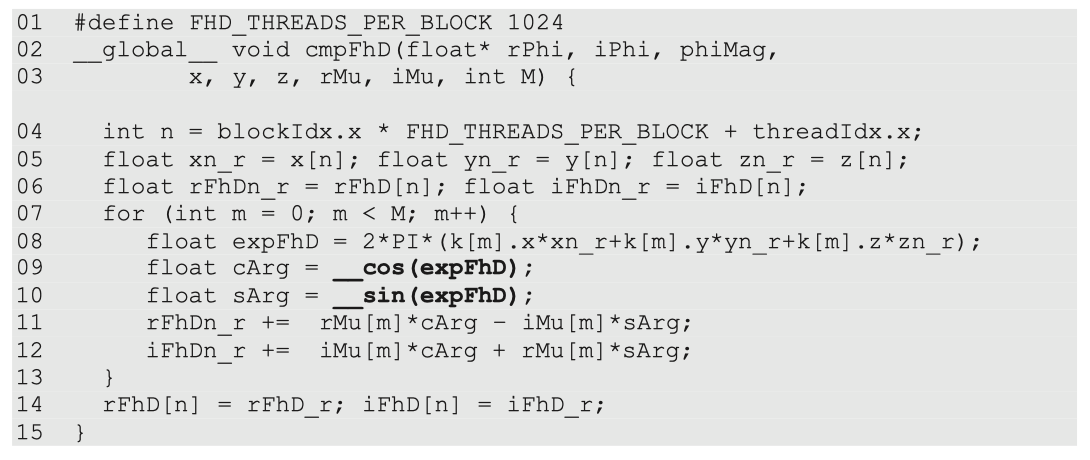
\includegraphics[width=0.9\textwidth]{figs/F17.17.png}
	\caption{\textit{使用硬件 \_\_sin() 和 \_\_cos() 函数。}}
\end{figure}

CUDA 提供数学函数的硬件实现,其吞吐量比相应的软件高得多。 
GPU 为 $\sin ($ ) 和 $\cos ()$ 等三角函数提供此类硬件实现的动机是提高图形应用中视角变换的速度。 
这些功能作为由SFU(特殊功能单元)执行的硬件指令来实现。 使用这些功能的过程非常简单。 
对于 cmpFhD 内核,我们需要做的是将 $\sin ()$ 和 $\cos ()$ 函数的调用
更改为其硬件版本:\_ $\sin ()$ 和 \_ $ \cos ()$(函数名前两个“\_”字符)。 
这些是编译器识别并翻译成 SFU 指令的内部函数。 
由于这些函数是在大量执行的循环体中调用的,因此我们预计这一更改将带来显着的性能改进。 生成的 cmpFhD 内核如图 17.17 所示。

\begin{figure}[H]
	\centering
	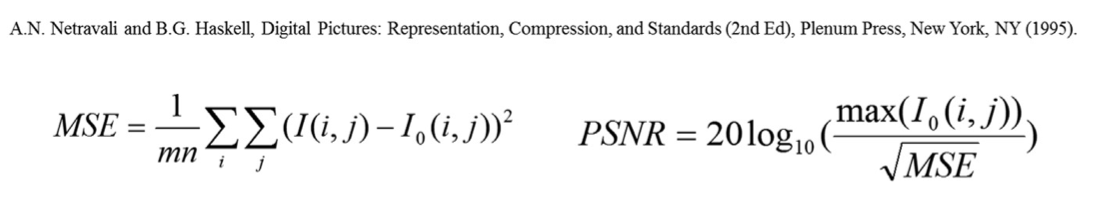
\includegraphics[width=0.9\textwidth]{figs/F17.18.png}
	\caption{\textit{用于验证硬件功能准确性的指标。 $I_0$ 是完美的图像。 $I$ 是重建图像。 PSNR 是峰值信噪比。}}
\end{figure}

但是,我们需要注意从软件功能切换到硬件功能的准确性降低。 
目前,硬件实现的准确性低于软件库(详细信息可在 CUDA C 编程指南中找到)。 
对于 MRI,我们需要确保硬件实现提供足够的精度,如图 17.18 中所定义。 
测试过程涉及虚构对象(有时称为幻像对象)的“完美”图像 $\left(\mathrm{I}_{0}\right)$。 
我们使用相反的过程来生成相应的合成的“扫描”kspace 数据。 然后合成的扫描数据由所提出的重建系统处理以生成重建图像(I)。 
然后将完美图像和重建图像中的体素值输入图 17.18 中的峰值信噪比 (PSNR) 公式中。

\begin{figure}[H]
	\centering
	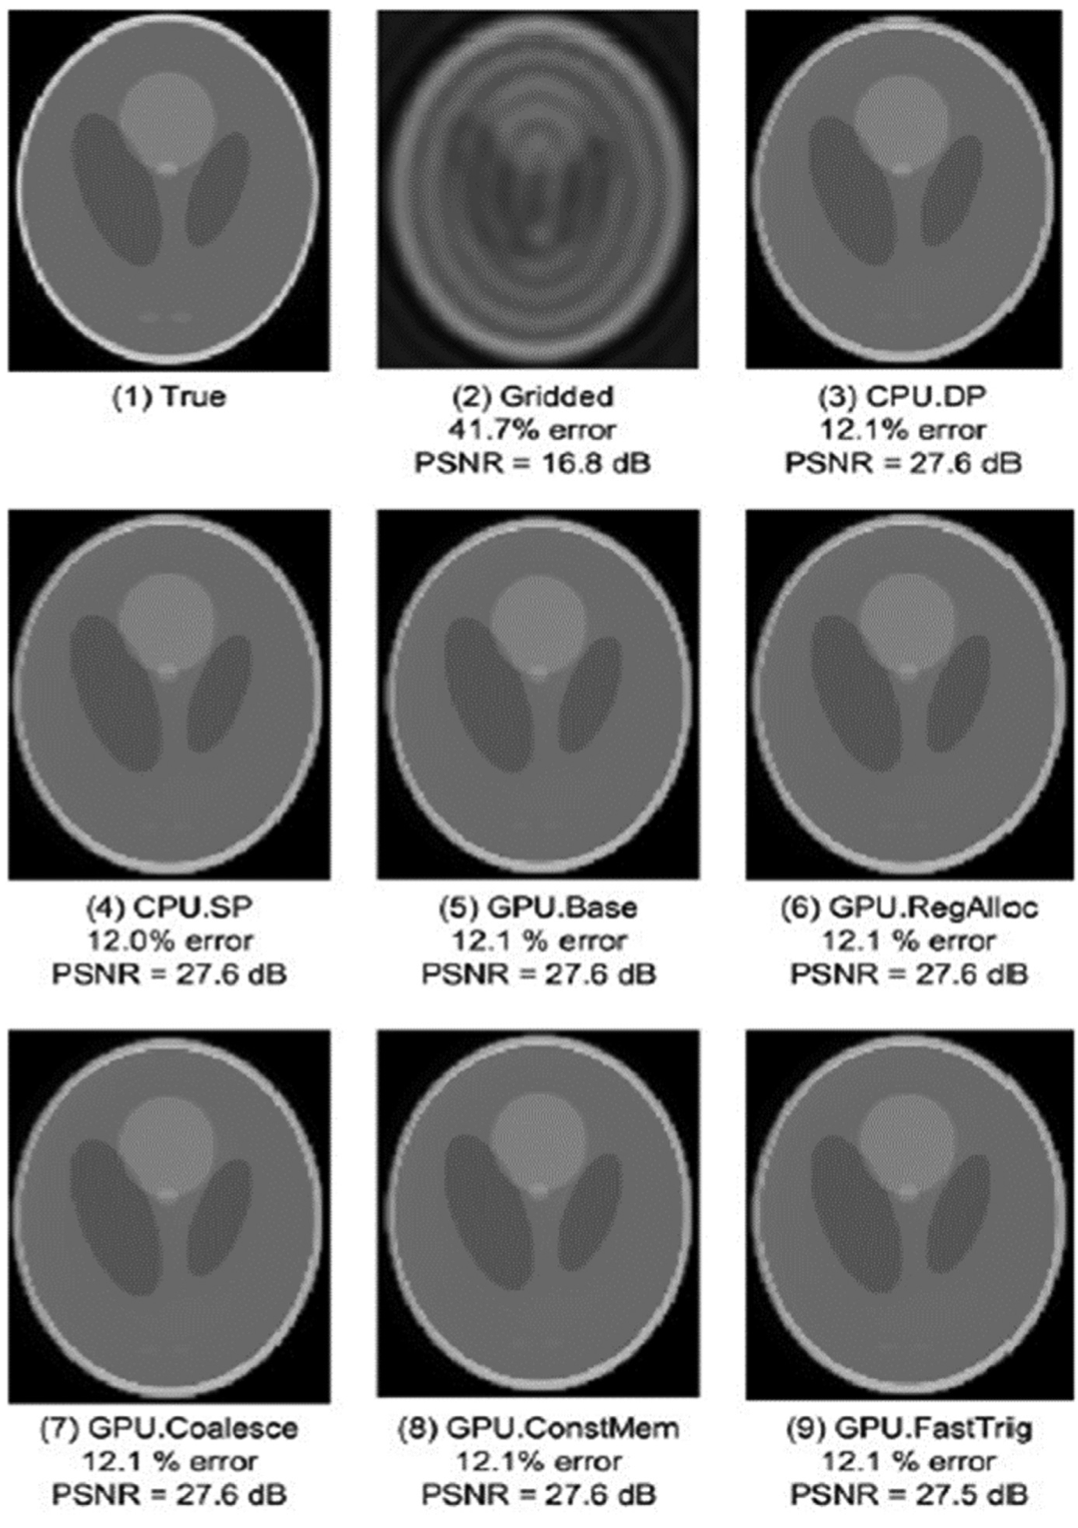
\includegraphics[width=0.9\textwidth]{figs/F17.19.png}
	\caption{\textit{验证不同 $F^H D$ 实现的浮点精度和准确度。}}
\end{figure}

通过测试的标准取决于图像的预期应用。 
在我们的案例中,我们与临床 MRI 专家合作,确保硬件功能引起的 PSNR 变化完全在其应用可接受的范围内。 
在医生使用图像来形成损伤印象或评估疾病的应用中,还需要对图像质量进行目视检查。 
图 17.19 显示了原始“真实”图像的视觉比较。 
然后,它表明 CPU 双精度和单精度实现实现的 PSNR 均为 $27.6 \mathrm{~dB}$,远高于应用程序可接受的水平。 
目视检查还表明,重建图像确实与原始图像很好地对应。

与简单的双线性插值网格/iFFT 相比,迭代重建的优势在图 17.19 中也很明显。 
使用简单网格/iFFT重建的图像的PSNR仅为$16.8 \mathrm{~dB}$,远低于通过迭代重建方法实现的$27.6 \mathrm{~dB}$的PSNR。 
对图 17.19(图像 2)中网格/iFFT 图像的目视检查表明,存在严重的伪影,可能会显着影响图像用于诊断目的的可用性。 
这些伪影不会出现在迭代重建方法的图像中。

当我们在 CPU 上从双精度算术转向单精度算术时,PSNR 没有明显下降,仍保持在 $27.6 \mathrm{~dB}$。 
当我们将三角函数从软件库移至硬件单元时,我们观察到 PSNR 的下降可以忽略不计,
从 $27.6 \mathrm{~dB}$ 到 $27.5 \mathrm{~dB}$。 PSNR 的轻微损失在应用的可接受范围内。 
目视检查确认重建图像与原始图像相比没有明显的伪影。

\subsubsection{第 4 步:实验性能调优}
到目前为止,我们还没有确定内核配置参数的适当值。 一个内核配置参数是每块的线程数。 
每个块需要使用足够数量的线程才能充分利用每个 SM 的线程容量。 
另一个内核配置参数是展开图 17.17(第 07 行)中的 for 循环体的次数。 
这可以通过使用“\#pragma unroll”后跟我们希望编译器在循环上执行的展开次数来设置。 
一方面,展开循环可以减少开销指令的数量,并可能减少处理每个 k 空间样本数据的时钟周期数。 
另一方面,过多的展开可能会增加寄存器的使用并减少 SM 中可容纳的块的数量。

请注意,这些配置的影响并不是相互隔离的。 增加一个参数值可能会使用原本可用于增加另一参数值的资源。 
因此,需要通过实验的方式联合评估这些参数。 可以有大量的组合可供尝试。 
在 $\mathrm{F}^{\mathrm{H}} \mathrm{D}$ 的情况下,通过系统地搜索所有组合并选择具有最佳测量运行时间的组合,
性能提高了约 $20 \%$,如下 与仅探索一些有希望的趋势的启发式调整搜索工作相比。 
柳等人。 (2008)提出了一种基于帕累托最优曲线的方法来筛选掉大多数较差的组合。

\subsection{总结}
在本章中,我们介绍了从顺序形式并行化和优化循环密集型应用程序(MRI 图像迭代重建)的关键步骤。 
我们从并行化的适当组织开始:分散方法与聚集方法。 
我们表明,从分散方法转换为聚集方法是避免原子操作的关键,原子操作会显着降低并行执行的性能。 
我们讨论了使聚集方法实现并行化所需的实用技术,即循环裂变和循环交换。

我们进一步介绍了优化技术的应用,例如将数组元素提升到寄存器中,对输入元素使用常量内存/缓存,
以及使用硬件功能来提高并行内核的性能。 正如我们所讨论的,从基本版本到最终优化版本,速度大约提高了 10 倍。

在并行化和优化之前,$\mathrm{F}^{\mathrm{H}} \mathrm{D}$ 曾经占据近 $100 \%$ 的执行时间。 
一个有趣的观察是,最终,CG 求解器(图 17.3 中的“find $\rho$”步骤)实际上比 $\mathrm{F}^{\mathrm{H}} \mathrm{D}$ 花费更多的时间。 
这是因为我们大幅加速了 $\mathrm{F}^{\mathrm{H}} \mathrm{D}$ 。 现在,任何进一步的加速都需要 CG 解算器的加速。 
成功并行化和优化后,$\mathrm{F}^{\mathrm{H}} \mathrm{D}$仅占 50\% 左右。 
另外 50\% 大部分花在 CG 解算器上。 这是并行化实际应用程序中众所周知的现象。 
由于成功的并行化工作会加速某些耗时的执行阶段,因此执行时间会被过去占据执行的无关紧要部分的其他阶段所支配。